\textbf{Ergebnis} (41 Wellenlängen, 58\,s): Die Transmission ist fast überall unter 0,5\,\%, steigt aber knapp oberhalb
der Plasmonenresonanz der ebenen Grenzfläche ($\lambda=1{,}3694$\um) auf 3,0\,\% bei $\lambda=1{,}385$\um{} -- rund dreißigmal so viel wie bei 1,5\um{}
(0,10\,\%), obwohl die Löcher mit 0,25\um{} Kantenlänge viel kleiner als die Wellenlänge sind. Gleichzeitig steigt die
Absorption von 2\,\% auf 10\,\%. Das Buch nennt $T\approx7{,}5\,\%$ bei 1,388\um; bei $N=6$ ist der Peak noch nicht
konvergiert.
\begin{figure}[h]
\centering
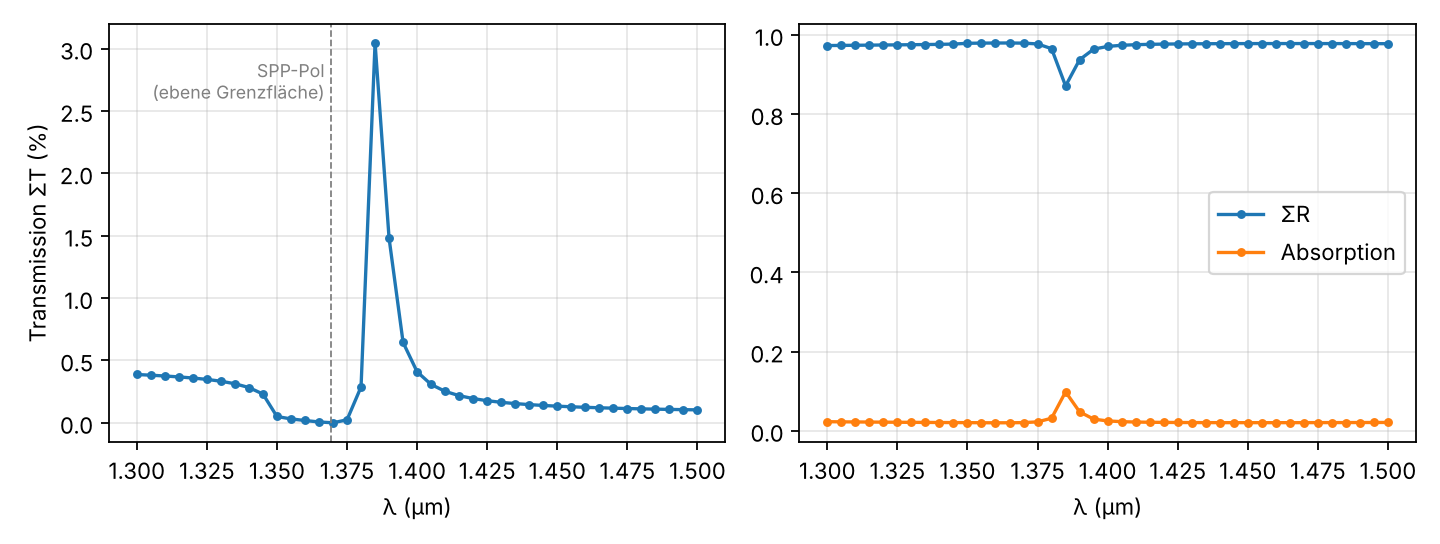
\includegraphics[width=\linewidth]{fig/v10_spec.png}
\caption{Silber-Lochgitter, $N_x=N_z=6$: Transmission (links), Reflexion und Absorption (rechts). Gestrichelt: Pol
des Oberflächenplasmons an der ebenen Silber-Luft-Grenzfläche.}
\end{figure}
